\documentclass{article}

\usepackage[spanish]{babel}
\usepackage[utf8x]{inputenc}
\usepackage{graphicx}

\begin{document}

% Título

\author{Daniel Izquierdo \\ \#08-86809}
\title{Examen Final \\ Web Semántica 2}
\date{14 de diciembre de 2009}
\maketitle

% Contenido

Con el rápido crecimiento que actualmente experimenta el ``Cloud of Linked
Data'' surgen muchas nuevas aplicaciones que involucran la recuperación de datos
de varias fuentes distintas, cada una con su propia estructura. Usuarios y
aplicaciones necesitan cada vez más tener la capacidad de evaluar muchas consultas
contra fuentes de datos heterogéneas. Las fuentes de datos se pueden
caracterizar por tener estructuras distintas y contener resultados parciales de
la consulta que se realiza. Además, escogiendo un criterio de calidad para las
fuentes, resulta que todas pueden tener valores distintos para los parámetros de
calidad. Para evaluar una consulta se deben conocer sus posibles reescrituras en
términos de las fuentes disponibles.

Por otra parte también existe la necesidad de componer servicios web
descubiertos para implementar realizar flujos de trabajo. Un usuario puede
definir un flujo de trabajo como una composición de servicios abstractos que son
implementados por servicios concretos. Al hacerlo, requiere conocer las maneras
de implementar los servicios abstractos con los concretos existentes. También
existen criterios de calidad que se deben tomar en cuenta a la hora de elegir
una implementación dada.

Precisamente por la explosión de datos y servicios que se vive en los momentos,
en ambos casos el espacio de soluciones a la pregunta de cuáles son las
reescrituras buscadas puede llegar a ser muy grande. Se requiere entonces de un
sistema que pueda resolver el problema de manera eficiente y escalable. El
proyecto que estoy desarrollando es un intento de crearlo.

La capacidad de escalar a números realistas de vistas (fuentes de datos o
servicios concretos) y sub-objetivos (pasos del flujo de trabajo) al momento de
reescribir las consultas dadas ya fue lograda por \ref{yarvelo}. Mi contribución
ha sido añadir la capacidad a esta solución de tomar en cuenta constantes en las
consultas y vistas, así como de manejar el concepto de rendimiento para
seleccionar las mejores reescrituras según los parámetros de calidad en un
problema dado.

A continuación muestro resultados experimentales que demuestran que la solución
desarrollada puede manejar tomando en cuenta constantes y parámetros de calidad.
Para evaluar el proyecto se ejecutaron pruebas con problemas reescritura de
flujos de trabajo en el área de vuelos y aerolíneas con las siguientes
características:

\begin{itemize}

\item Servicio abstracto {\it vuelo(x,y,a)} que relaciona las ciudades $x$ e $y$
si hay un vuelo de la aerolínea $a$ entre ellas.

\item Consultas que retornan escalas para vuelos entre una ciudad $a$ y otra
ciudad $b$ dadas, con la condición de que todos los vuelos usan la misma
aerolínea. Tienen la forma:

$$
q(x_0,x_1,\ldots,x_{n-1}) :- vuelo(a,x_0,z),\, vuelo(x_0,x_1,z), \ldots, vuelo(x_{n-2},x_{n-1},z), vuelo(x_{n-1},b,z)
$$

\item Servicios concretos $v_A$ que retornan vuelos con una aerolínea dada. Por
ejemplo:

$$
v_{\mathrm{CO}} :- vuelo(x,y,\mathrm{CO})
$$

\end{itemize}

Los parámetros variables en los experimentos fueron el número de vistas (de 5 a
80 en incrementos de 5) y el
número de objetivos de las consultas (de 2 a 5). Podemos ver los resultados en la
figura \ref{grafico:plot1}.

\begin{figure}[h!]
  \caption{Resultados del primer experimento}
  \centering
   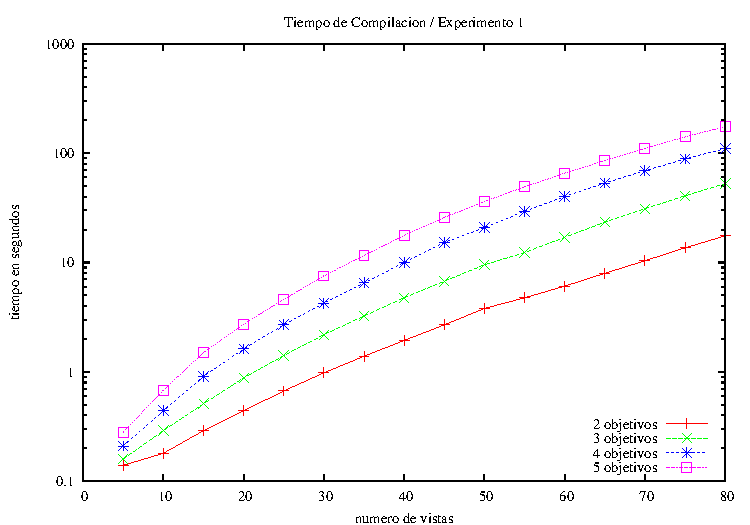
\includegraphics[width=0.5\textwidth]{plot1}
  \label{grafico:plot1}
\end{figure}

A partir de estos resultados tenemos observaciones importantes. En primer lugar
se nota la progresión polinomial de los tiempos de ejecución, por lo que podemos
hablar de alta eficiencia, al menos para este tipo de problemas. Además vemos
tiempos muy razonables para instancias con tamaños de la vida real. El caso más
grande tiene ochenta aerolíneas y vuelos con cinco escalas --números bastante
ajustados a lo que se vería en una agencia de viajes, por ejemplo-- fue resuelto
en menos de cuatro minutos. Cabe acotar que, por la arquitectura de la solución
desarrollada, se puede ``compilar'' una instancia del problema de manera de
satisfacer múltiples consultas sobre la misma instancia pero con parámetros de
calidad distinto de forma muy veloz; para el caso más grande toma menos de un
segundo resolver una consulta una vez obtenida la versión compilada.

A pesar de los buenos resultados, hay que aclarar que el sistema desarrollado
está limitado en cuanto a escalabilidad a miles de vistas y decenas de objetivos
de consulta. Al realizar pruebas con problemas de tamaño mucho mayor se
encontraron tiempos de ejecución inmanejablemente grandes. Parte del trabajo
futuro sobre el tema se puede realizar en la dirección de hacer accesible
instancias de problemas con estos tamaños.

\end{document}
